\documentclass[10pt]{report}
\renewcommand{\thesection}{\Roman{section}} 
\renewcommand{\thesubsection}{\thesection.\Roman{subsection}}

\renewcommand{\baselinestretch}{1.5}

\setlength{\topmargin}{-2cm}
\setlength{\oddsidemargin}{0cm}
\setlength{\textheight}{24cm}
\setlength{\textwidth}{16cm}

\usepackage{amsmath}
\usepackage{bm}
\usepackage{csvsimple}
\usepackage{booktabs}
\usepackage{graphicx}

\begin{document}

\title{%
  Machine Learning Engineer Nanodegree \\
  \large Capstone Project}
\author{Dennis P. F.}
\date{December 14th, 2016}
\maketitle

\section{Definition}
\subsection*{Project Overview}
Stock price prediction is a very basic and important operation in financial entities like hedge funds, mutual funds and exchange traded funds. Performance of these financial institutions depend highly on the degree of success of this prediction. Many works in the past have used machine learning techniques like Linear Discriminant Analysis(LDA), K-nearest neighbor(KNN), Gaussian Process, Support Vector Machines(SVM), Neural Networks(ANN), Random Forest and Naive Bayes\cite{Ou2009}\cite{Patel2015}. In this project a blend of two instances of Adaboost ensemble regression with Linear regression and KNN as base algorithms is used to train on daily prices/volume data for a selected number of stocks of S\&P 500\cite{sp500} index obtained from Yahoo Finance. The final model is then used to make a 5-day forecast of returns of the selected stocks.

\subsection*{Problem Statement}
The goal is to make a 5-day forecast of returns of N current stocks of S\&P 500 index which were first added before 2006-01-01 purely based on Technical Analysis features like past m day’s Adjusted close prices, Simple Moving Average(SMA), Rolling Standard Deviation(RSD), Bollinger-Bands(BB)\cite{bollingerbands} and Momentum of the adjusted close prices and also based on the daily Volume of each stock. Mathematically the aim can be written as :\\
Estimate the functions $F_i$ $\forall i \in [0,N-1]$ such that\\
\begin{align*}
\bm{R^{forecast}_{i}} &= \bm{F_i}(\bm{P_i}, \bm{SMA_i}, \bm{RSD_i}, \bm{BBScore_i}, \bm{MScore_i},\bm{ Volume_i})\\
\text{where}\\
\bm{R^{forecast}_{i}} &= [ \frac{P_{i, t+1}}{P_{i, t}} - 1, \frac{P_{i, t+2}}{P_{i, t}} - 1, \frac{P_{i, t+3}}{P_{i, t}} - 1, \frac{P_{i, t+4}}{P_{i, t}} - 1, \frac{P_{i, t+5}}{P_{i, t}} - 1] \\
\bm{P_i} &= [ P_{i, t}, P_{i, t-1}, ..., P_{i, t-m+1} ] \\
\bm{SMA_i} &= [ SMA_{i, t}, SMA_{i, t-1}, ..., SMA_{i, t-m+1} ]\\
\bm{RSD_i} &= [ RSD_{i, t}, RSD_{i, t-1}, ..., RSD_{i, t-m+1} ]\\
\bm{BBScore_i} &= [ BBScore_{i, t}, BBScore_{i, t-1}, ..., BBScore_{i, t-m+1} ]\\
\bm{MScore_i} &= [ MScore_{i, t}, MScore_{i, t-1}, ..., MScore_{i, t-m+1} ]\\
\bm{Volume_i} &= [ Volume_{i, t}, Volume_{i, t-1}, ..., Volume_{i, t-m+1} ]
\end{align*}
$P_{i,t}$ is the $t^{th}$ day's adjusted-close\cite{adjclose} price of $i^{th}$ stock from the N selected stocks of current S\&P 500 index sorted alphabetically by ticker.\\
$SMA_{i,t}$ is given by $\frac{1}{10}\sum_{j=t-9}^{t} P_{i,j}$ which is the 10 day simple moving average of the $i^{th}$ stock.\\
$RSD_{i,t}$ is given by $\sqrt{\frac{1}{10}\sum_{j=t-9}^{t} \left( P_{i,j} - SMA_{i,j}\right)^2}$ which is the 10 day rolling standard deviation of the $i^{th}$ stock.\\
$BBScore_{i,t}$ is given by $\frac{P_{i,t} - SMA_{i,t}}{2 RSD_{i,t}}$ which is the Bollinger bands score of $i^{th}$ stock as introduced in \cite{mlfortrading} \\
$MScore_{i,t}$ is given by $\frac{P_{i,t}}{P_{i, t-9}}$ which is the momentum score for $i^{th}$ stock as introduced in \cite{mlfortrading}\\
$Volume_{i,t}$ is the $t^{th}$ day's volume of the $i^{th}$ stock.\\
\\
The tasks involved in the solution are as follows:
\begin{enumerate}
\item Retrieve the list of tickers in current S\&P 500 index filter out those which stocks which got added after 2006-01-01
\item Get the historical price-volume data in the range [2006-01-01 to 2016-12-10] for each of the selected tickers from Yahoo Finance webservice.
\item Reshape the downloaded data to form a dataset of the form: 
\begin{align*}
[&(feature_1, feature_2, ..., feature_n, target)_{t=0},\\
 &(feature_1, feature_2, ..., feature_n, target)_{t=1},\\
 &...\\
 &(feature_1, feature_2, ..., feature_n, target)_{t=S}]\\
\end{align*} where S is the number of points in the dataset.
\item Split the dataset to train set, validation set and test set in the proportion 80:10:10 such that train set has the oldest 80\% of dataset w.r.t date, and validation set has next 10\% and test set has the final/newest 10\% of the dataset. This is to avoid any look-ahead bias in the model that is going to be trained and tuned.
\item Train a regression model on the train set and tune the parameters of the model using the validation set.
\item Train the model using combined train + validation set using the best parameters obtained in previous step.
\item Use the above model to evaluate in the test set.
\end{enumerate}
The model thus produced is expected to be useful in making reasonably accurate future 5-day predictions.

\subsection*{Metrics}
A suitable evaluation metric for the project is $R^2$ score or coefficient of determination\cite{r2score} since it is a regression problem. It reflects how well future samples are likely to be predicted by the
model. It produces a score in the range $(-\infty, 1]$. $R^2$ score = 1 indicate best performance and those closer to zero and below indicate poor performance. A model that just returns the mean of target variables as output will have $R^2$ score = 0. $R^2$ evaluation metric takes estimated target sample vector $\hat{Y}$ and corresponding ground truths vector Y each of length M and computes the score as :\\
\\
$R^2\left(Y, \hat{Y}\right) = 1 - \frac{\displaystyle\sum_{k=0}^{M-1} \left(Y_k - \hat{Y}_k\right)^2}{\displaystyle\sum_{k=0}^{M-1} \left(Y_k - \bar{Y}\right)^2}$\\
where\\
$\bar{Y} = \frac{1}{M} \displaystyle\sum_{k=0}^{M-1} Y_k$
\\
\\
Since there are N stocks and the model needs to output 5 continuous valued real numbers (5-day forecasts) per each stock, the model would consist of $5 \times N$ single target regressions, hence when $R^2$ evaluation metric is used to evaluate each regression individually, there would be $5 \times N$ $R^2$ values. As it is always easier to work with a single performance metric, the individual $R^2$ scores are averaged with equal weightage :\\
\begin{align*}
\text{Validation set performance metric} &= \frac{1}{5N} \displaystyle\sum_{i=0}^{N-1} \displaystyle\sum_{j=1}^{5} R^2\left(Y_{i,j}^{valid}, \hat{Y}_{i,j}^{valid}\right)\\
\text{Test set performance metric} &= \frac{1}{5N} \displaystyle\sum_{i=0}^{N-1} \displaystyle\sum_{j=1}^{5} R^2\left(Y_{i,j}^{test}, \hat{Y}_{i,j}^{test}\right)
\end{align*}
where $Y_{i,j}^{valid}$ and $\hat{Y}_{i,j}^{valid}$ are the actual and predicted returns respectively in the validation set for $i^{th}$ stock on the day T+j where T is the supposed current date
and similarly $Y_{i,j}^{test}$ and $\hat{Y}_{i,j}^{test}$ are the actual and predicted returns respectively in the test set for $i^{th}$ stock on the day T+j.

\section{Analysis}
\subsection*{Data Exploration}
First step in getting data is to parse the wikipedia webpage\cite{sp500} to get a list of tickers that were first added before 2006-01-01. Next step is to use the Yahoo Finance webservice to get historical prices and volume for each of the selected tickers from 2006-01-01 to 2016-12-10. Whole of this process can be done by invoking the script fetchdata.py as :\\
\texttt{\$ cd src\\
\$ python fetchdata.py}\\
Historical data for each ticker is downloaded to \texttt{data/} dir as a csv file. There are 2755 trading days between 2006-01-01 and 2016-12-10, so those stocks which have traded for all these days will have 2755 rows in them. For example AAPL.csv has 2755 data rows excluding the header. However there are tickers that have lesser number of rows :\\
\texttt{\$ wc -l *.csv | sort -n  | head\\
     130 NEE.csv\\
     372 WRK.csv\\
    2505 SE.csv\\
    2568 WU.csv\\
    2620 WYN.csv\\
    2756 AAPL.csv\\
    2756 ABC.csv\\
    2756 ABT.csv\\
    2756 A.csv\\
    2756 ADBE.csv}\\
These tickers [\textbf{NEE, WRK, SE, WU, WYN}] are excluded from further use in the project. The number of stocks after exclusion of these stocks is 308.
Every csv file has the columns [Date, Open, High, Low, Close, Volume, Adj Close], from this only the columns Date, Volume and Adj Close are used in the project to compute features/targets and none of the columns has missing values for any stock.
The following steps are done to these selected columns to get the needed features :
\begin{enumerate}
\item Sort the raw data with respect to Date column in ascending order(oldest date to newest date).
\item Compute the features [SMA, RSD, BBScore, MScore] as described in the problem statement section.
\item Compute natural logarithm of the Volume field as Volume is typically a large positive number. Taking log will make its distribution approximately normal.
\end{enumerate}
\textbf{Table. 1} Table showing the basic statistics of the relevant features for AAPL stock.\\
\csvautobooktabular{AAPL_desc.csv}
\\
\\
Note that the count of all the features is only 2745, that is because oldest 10 rows will not have SMA, RSD and MScore values as they are rolling features which look back 10 days.\\
\subsection*{Exploratory Visualization}
The exploratory visualization of a particular stock can be seen by invoking the \texttt{explore.py} script as :\\
\texttt{\$ cd src\\
\$ python explore.py}\\
It produces the histogram plots of all features used and also the variation of all normalized features as a function of date.\\
\textbf{Fig.1} Set of histograms of the features Adjusted-Close price(Adj Close), Bollinger Bands score(BB), Natural logarithm of volume (LogVolume), Momentum score(MOM), Rolling standard deviation(RSD), Simple moving average(SMA). Adj Close and SMA have similar histograms as expected. MOM has an approximate normal distribution with $mean = 1.0$ BB's histogram indicate a dominant positive mode indicating frequent price movements above SMA. RSD has an approximate lognormal distribution.\\
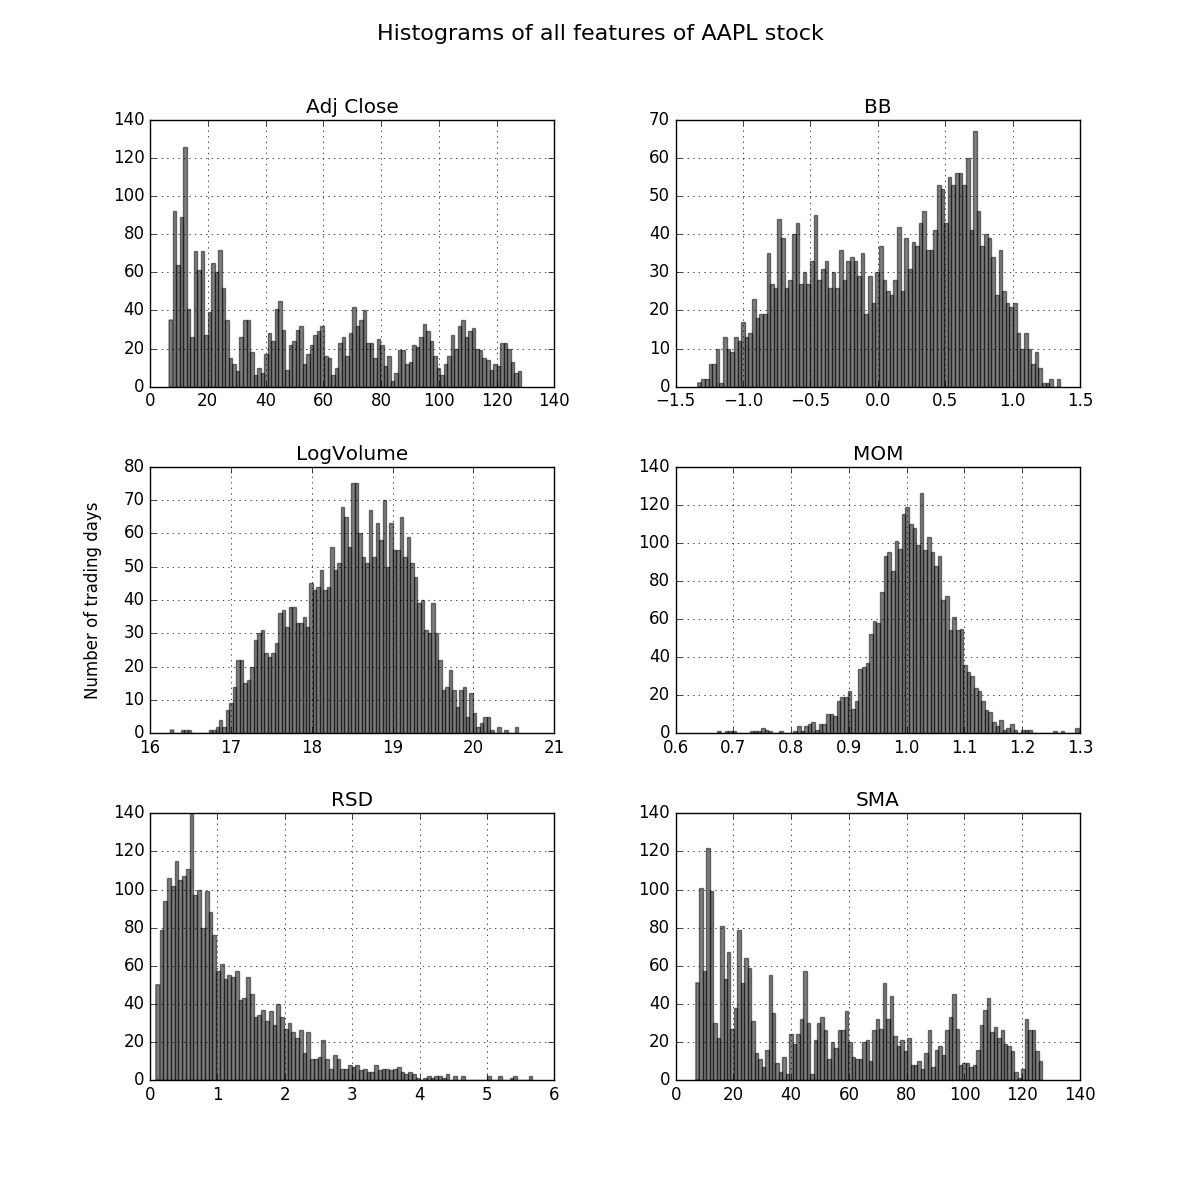
\includegraphics[width=11cm]{plots/histograms.png}\\
\textbf{Fig.2} Set of plots showing the timeseries of normalized features for AAPL stock with date range [2006-01-18 to 2007-03-28]. Top plot indicate the timeseries of normalized Adjusted close price, SMA and RSD. Middle plot shows timeseries of Adjusted close, BBscore, MScore and the bottom plot shows the timeseries of Adj Close and LogVolume.\\
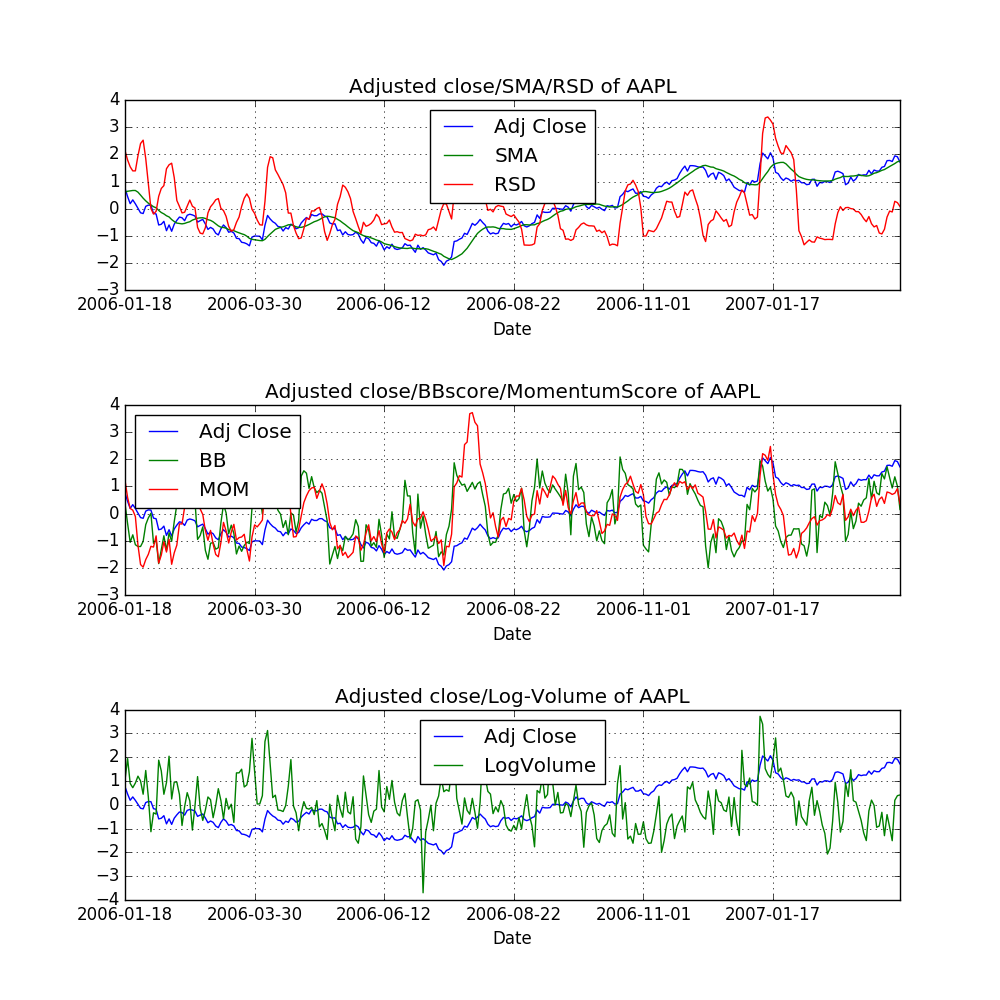
\includegraphics[width=12cm]{plots/allplots.png}\\
It can be seen from the first timeseries plot that SMA is a smoother version of the adjusted close price and lags a bit behind it. RSD value becomes high whenever there is a large instantaneous variation in adj close from SMA. Momentum score(MOM) shows that often when it is very high the immediate future prices are going to go up and very low values of MOM indicate a immediate future price drop. Volume time series shows that it goes up usually due to a large variation of price in a small time window. Generally visual inferences from timeseries plots are difficult apart from some very obvious cues in price movements. Next, correlation of different features with the future prices are examined to get a more clear view although, correlation uncovers only the degree of linear relationship between variables.\\
\\
\textbf{Fig.3} Set of bar plots showing the Pearson correlation coefficient of target returns(T+1, T+2, T+3, T+4, T+5) with all features.\\
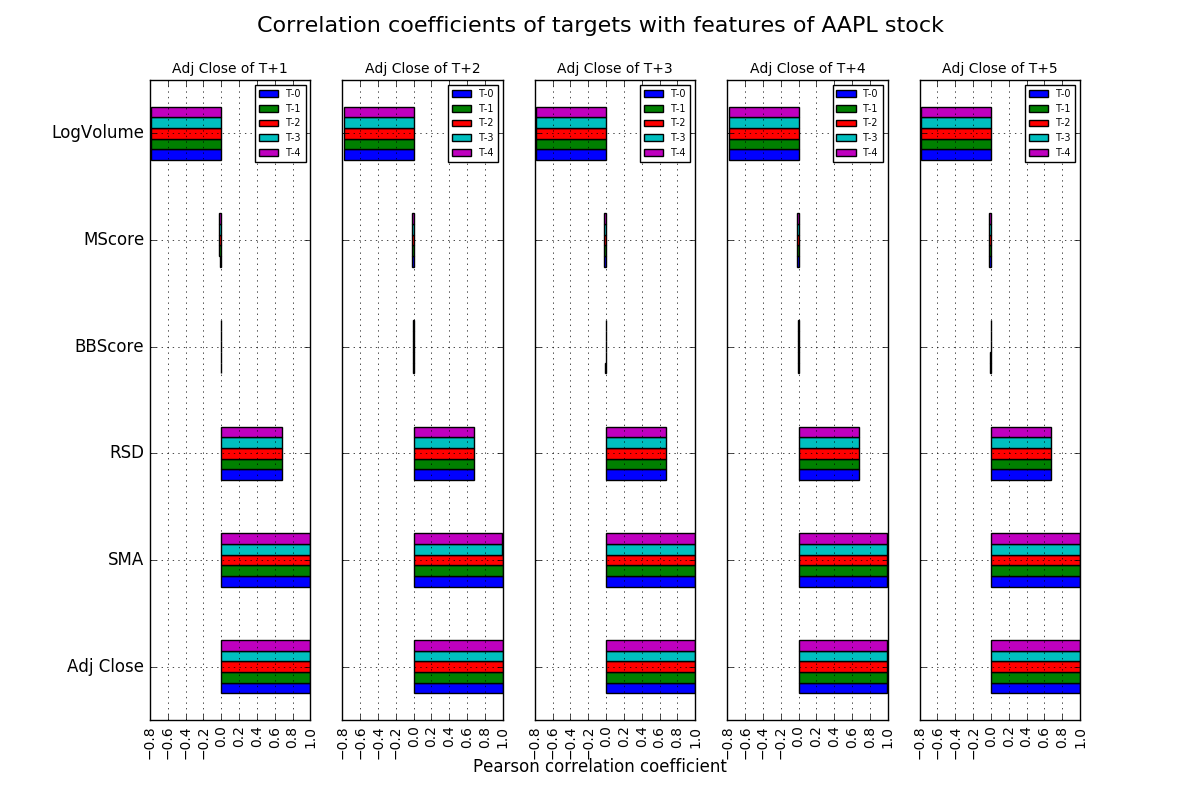
\includegraphics[width=12cm]{plots/corrcoeffs.png}\\
Generally all correlation coefficients here are small in magnitude as is the case with any financial return regressors. It can be seen that RSD has relatively highest absolute correlation with future returns. Since correlation-measure indicates the degree of linear relationship between variables, a simple Linear Regression would be able to take advantage of these relationships to do prediction. Even though the the correlation coefficients of LogVolume and MScore with targets are very low, a nonlinear regression may be able to make use of these features to make predictions better than the linear models.
\subsection*{Algorithms and Techniques}
% This project focus on using AdaBoost ensemble regression method with different base estimators. AdaBoost lets the use of several ensembles of a weak learner to produce a better performing meta-model on the given dataset. The following models are evaluated on the dataset to do 5-day forecast of adjusted-close prices.
% \begin{enumerate}
% \item AdaBoost Regressor with KNN as base regression algorithm. The parameters to tune are K(The number of nearest neighbors in KNN), n\_estimators(number of estimators for AdaBoost).
% \item AdaBoost Regressor with Linear regression as base algorithm. The parameters to tune is n\_estimators (number of estimators for AdaBoost).
% \end{enumerate}
% The parameters of these models are tuned by looking at the performance in the validation set. Since the dataset is small enough as shown in Data Processing section, whole of it is held in RAM during the process of training, parameter tuning with validation set and evaluation in the test set.
\subsection*{Benchmark}
Ordinary least squares Linear Regression is used as the benchmark model. This model produce an average $R^2$ score of $-0.169495$ on the dataset of the selected stocks[AAPL, HIG, MRK, PLD, XOM].
\section{Methodology}
\subsection*{Data Processing}
To evaluate each prediction model, only a random sample of 5 stocks[AAPL, HIG, MRK, PLD, XOM] is used without much loss of generality. First step is to form a dataset in the form ([set of features], target). A single row in this dataset for each date for a particular stock has the features :
\begin{enumerate}
\item Adj Close for past $m=5$ days including current date i.e., the date of dataset row.
\item SMA for past $m=5$ days including current date.
\item RSD for past $m=5$ days including current date.
\item BBScore for past $m=5$ days including current date.
\item MScore for past $m=5$ days including current date.
\item LogVolume for past $m=5$ days including current date.
\end{enumerate}
The target for each row is the vector of next 5 day's returns. Number of rows in the dataset is $2736$ because of 5-day look back for computing features including current day and 5-day forecast. Number of features in each example is $6 \times 5 = 30$ and the number of targets per each example is $5$. The amount of memory required to load the dataset assuming 8-bytes for a floating point number is $ 308 \times 2736 \times ( 30  +  5 ) \times 8 = 235,952,640 \text{ Bytes} \approx 225.02 \text{ MB}$. So the whole dataset can be loaded in memory for any modern machine.

Next step is to divide the dataset to training, validation set and test set in the proportion 80:10:10. Before applying any learning algorithm, the features are normalized using mean and standard deviation:
$feature_i^{normalized} = \frac{feature_i - mean(feature_i)}{stddev(feature_i)}$
\subsection*{Implementation}

\section{Results}

\section{Conclusion}

\begin{thebibliography}{}

\bibitem{Ou2009}
Ou, Phichhang, and Hengshan Wang. "Prediction of stock market index movement by ten data mining techniques." Modern Applied Science 3.12 (2009): 28
\bibitem{Patel2015}
Patel, Jigar, et al. "Predicting stock and stock price index movement using trend deterministic data preparation and machine learning techniques.” Expert Systems with Applications 42.1 (2015): 259-268
\bibitem{adjclose}
Adjusted close price - www.investopedia.com/terms/a/adjusted\_closing\_price.asp
\bibitem{bollingerbands}
Bollinger bands - en.wikipedia.org/wiki/Bollinger\_Bands
\bibitem{mlfortrading}
Machine Learning for Trading Course by Udacity - www.udacity.com/course/machine-learning-for-trading--ud501
\bibitem{sp500}
S\&P500 constituents - en.wikipedia.org/wiki/List\_of\_S\%26P\_500\_companies
\bibitem{r2score}
R2 score - scikit-learn.org/stable/modules/model\_evaluation.html\#r2-score

\end{thebibliography}

\end{document}